\subsection{Etapa de Ideação}


\subsubsection{Backend}

A modelagem do banco de dados sempre será atualizado conforme a necessidade de implementação e conforme forem surgindo as dificuldades de implementação.

\begin{figure}[!htb]
    \centering
    \caption[short]{Modelagem do banco de dados}
    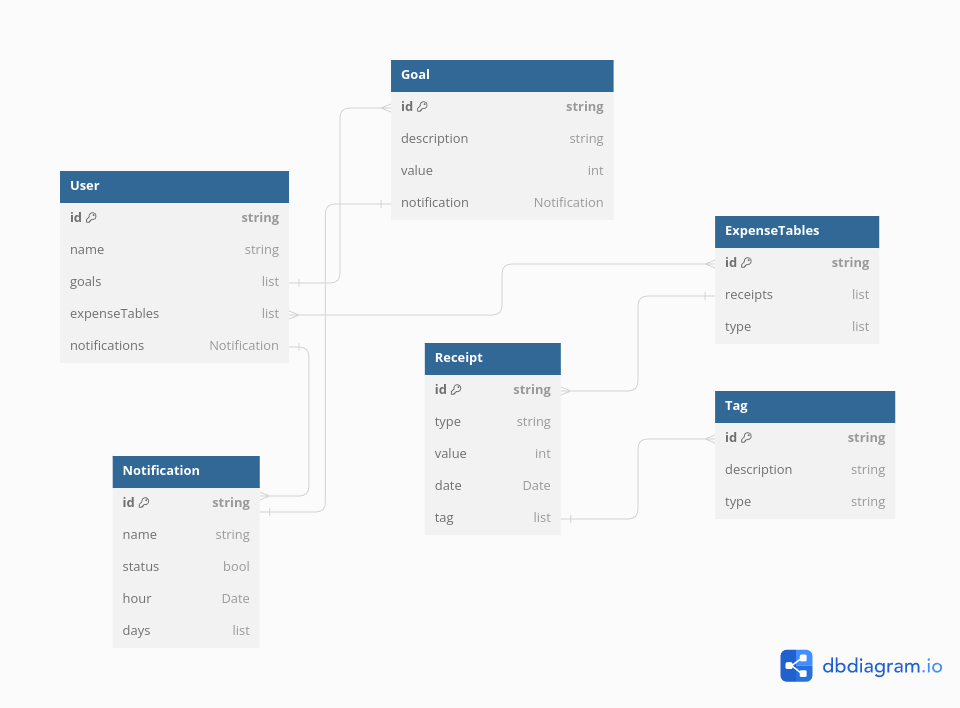
\includegraphics[scale=0.4]{images/backend_model.png}
\end{figure}


\subsubsection{Frontend}

O frontend utilizado foi a partir de um modelo pronto desenvolvido para mobile que será adaptado para uma interface web, visto que um dos requisitos das pessoas entrevistadas era ter uma visão completa de todos os meses, e para isso seria muito melhor ser mostrado dentro de uma tela de computador.

Portanto, todo o design do frontend foi baseado no \textit{Montra}, uma design desenvolvido, especificamente, para mobile.


\noindent{\textit{\textbf{OBS:} O design pode ser observado a partir da figura 3.}}